% file: chap6.tex

\chapter{深度学习}
\label{ch:Deeplearning}

在\hyperref[ch:WhyHardToTrain]{上一章},我们学习了深度神经网络通常比浅层神经网络
更加难以训练。我们有理由相信,若是可以训练深度网络,则能够获得比浅层网络更加强大
的能力,但是现实很残酷。从上一章我们可以看到很多不利的消息,但是这些困难不能阻止
我们使用深度神经网络。本章,我们将给出可以用来训练深度神经网络的技术,并在实战中
应用它们。同样我们也会从更加广阔的视角来看神经网络,简要地回顾近期有关深度神经网
络在图像识别、语音识别和其他应用中的研究进展。然后,还会给出一些关于未来神经网络
又或人工智能的简短的推测性的看法。

这一章比较长。为了更好地让你们学习,我们先粗看一下整体安排。本章的小结之间关联并
不太紧密,所以如果读者熟悉基本的神经网络的知识,那么可以任意跳到自己最感兴趣的部
分。

\hyperref[sec:convolutional_networks]{本章主要的部分}是对最为流行神经网络之一的深
度卷积网络的介绍。我们将细致地分析一个使用卷积网络来解决 MNIST 数据集的手写数字识
别的例子(包含了代码和讲解):
\begin{center}
  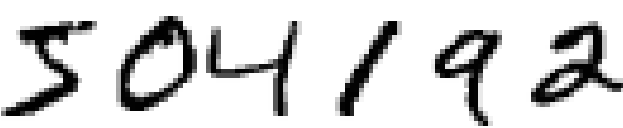
\includegraphics[width=64pt]{digits}
\end{center}

我们将从浅层的神经网络开始来解决上面的问题。通过多次的迭代,我们会构建越来越强大
的网络。在这个过程中,也将要探究若干强大技术:卷积、pooling、使用GPU来更好地训练、
训练数据的算法性扩展(避免过匹配)、dropout 技术的使用(同样为了防止过匹配现象)、
网络的 ensemble 使用 和 其他技术。最终的结果能够接近人类的表现。
在 10,000 幅 MNIST 测试图像上 —— 模型从未在训练中接触的图像 —— 该系统最终能够将其
中 9,967 幅正确分类。这儿我们看看错分的 33 幅图像。注意正确分类是右上的标记;系统
产生的分类在右下:
\begin{center}
  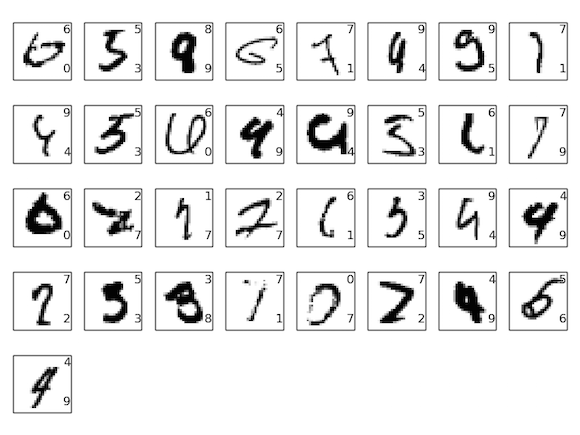
\includegraphics[width=.75\textwidth]{ensemble_errors}
\end{center}

可以发现,这里面的图像使对于人类来说都是非常困难区分的。例如,在第一行的第三幅图。
我看的话,看起来更像是 “9” 而非 “8”,而 “8” 却是给出的真实的结果。我们的网
络同样能够确定这个是 “9”。这种类型的“错误”最起码是容易理解的,可能甚至值得我
们赞许。最后用对最近使用深度(卷积)神经网络在图像识别上的研究进展作为关于图像识
别的讨论的总结。

本章剩下的部分,我们将会从一个更加宽泛和宏观的角度来讨论深度学习。概述一些神经网
络的其他模型,例如 RNN 和 LSTM 网络,以及这些网络如何在语音识别、自然语言处理和其
他领域中应用的。最后会试着推测一下,神经网络和深度学习未来发展的方向,会
从 intention-driven user interfaces 谈谈深度学习在人工智能的角色。这章内容建立在
本书前面章节的基础之上,使用了前面介绍的诸如 BP、规范化、softmax 函数,等等。然而,
要想阅读这一章,倒是不需要太过细致地掌握前面章节中内容的所有的细节。当然读完第一
章关于神经网络的基础是非常有帮助的。本章提到第二章到第五章的概念时,也会在文中给
出链接供读者去查看这些必需的概念。

需要注意的一点是,本章所没有包含的那一部分。这一章并不是关于最新和最强大的神经网
络库。我们也不是想训练数十层的神经网络来处理最前沿的问题。而是希望能够让读者理解
深度神经网络背后核心的原理,并将这些原理用在一个 MNIST 问题的解决中,方便我们的理
解。换句话说,本章目标不是将最前沿的神经网络展示给你看。包括前面的章节,我们都是
聚焦在基础上,这样读者就能够做好充分的准备来掌握众多的不断涌现的深度学习领域最新
工作。本章仍然在Beta版。期望读者指出笔误,bug,小错和主要的误解。如果你发现了可疑
的地方,请直接联系 mn@michaelnielsen.org。

\section{介绍卷积网络}
\label{sec:convolutional_networks}

在前面的章节中,我们教会了神经网络能够较好地识别手写数字:
\begin{center}
  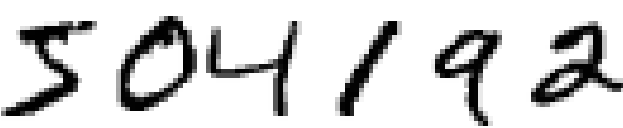
\includegraphics[width=64pt]{digits}
\end{center}

我们使用了全连接的邻接关系的网络来完成这个工作。即,网络中的神经元与相邻的层上的
每个神经元均连接:
\begin{center}
  \includegraphics{tikz41}
\end{center}

特别地,对输入图像中的每个像素点,我们将其光强度作为对应输入层神经元的值。对
于 $28 \times 28$ 像素的图像,这意味着我们的网络有
$784$($= 28 \times 28$)个输入神经元。我们然后训练网络的权重和偏差,使得网络输出
能够 —— 如我们希望地 —— 正确地辨认输入图像:'0', '1', '2', ..., '8', or '9'。

我们之前地网络工作得相当好:we've obtained a classification accuracy better than
98 percent, using training and test data from the MNIST handwritten digit data
set. But upon reflection, it's strange to use networks with fully-connected
layers to classify images. The reason is that such a network architecture does
not take into account the spatial structure of the images. For instance, it
treats input pixels which are far apart and close together on exactly the same
footing. Such concepts of spatial structure must instead be inferred from the
training data. But what if, instead of starting with a network architecture
which is tabula rasa, we used an architecture which tries to take advantage of
the spatial structure? In this section I describe convolutional neural
networks\footnote{The origins of convolutional neural networks go back to the
  1970s. But the seminal paper establishing the modern subject of convolutional
  networks was a 1998 paper, "Gradient-based learning applied to document
  recognition", by Yann LeCun, Léon Bottou, Yoshua Bengio, and Patrick
  Haffner. LeCun has since made an interesting remark on the terminology for
  convolutional nets: "The [biological] neural inspiration in models like
  convolutional nets is very tenuous. That's why I call them 'convolutional
  nets' not 'convolutional neural nets', and why we call the nodes 'units' and
  not 'neurons' ". Despite this remark, convolutional nets use many of the same
  ideas as the neural networks we've studied up to now: ideas such as
  backpropagation, gradient descent, regularization, non-linear activation
  functions, and so on. And so we will follow common practice, and consider them
  a type of neural network. I will use the terms "convolutional neural network"
  and "convolutional net(work)" interchangeably. I will also use the terms
  "[artificial] neuron" and "unit" interchangeably.}. These networks use a
special architecture which is particularly well-adapted to classify
images. Using this architecture makes convolutional networks fast to
train. This, in turns, helps us train deep, many-layer networks, which are very
good at classifying images. Today, deep convolutional networks or some close
variant are used in most neural networks for image recognition.

卷积神经网络采用了三种基本概念:\emph{局部感受野\index{局部感受野}(local
  receptive fields\index{local receptive fields})},\emph{共享权重\index{共享权
    重}(shared weights\index{shared weights})},和\emph{混合储存\index{混合储
    存}(pooling\index{pooling})}。让我们逐个看下:\\

\textbf{局部感受野:} 在之前看到的全连接层的网络中,输入被描绘成纵向排列的神经元。
但在一个卷积网络中,把输入看作是一个 $28 \times 28$ 的方形排列的神经元更有帮助,
其值对应于我们用作输入的 $28 \times 28$ 的像素光强度:
\begin{center}
  \includegraphics{tikz42}
\end{center}

和通常一样,我们把输入像素连接到一个隐藏神经元层。但是我们不会把每个输入像素连接
到每个隐藏神经元。相反,我们只是把输入图像进行小的,局部区域的连接。

说的确切一点,第一个隐藏层中的每个神经元会连接到一个输入神经元的一个小区域,例如,
一个 $5 \times 5$ 的区域,对应于 $25$ 个输入像素。所以对于一个特定的隐藏神经元,
我们可能有看起来像这样的连接:
\begin{center}
  \includegraphics{tikz43}
\end{center}

这个输入图像的区域被称为隐藏神经元的\emph{局部感受野}。它是输入像素上的一个小窗口。
每个连接学习一个权重。而隐藏神经元同时也学习一个总的偏差。你可以把这个特定的隐藏
神经元看作是在学习分析它的局部感受野。

我们然后在整个输入图像上交叉移动局部感受野。对于每个局部感受野,在第一个隐藏层中
有一个不同的隐藏神经元。为了正确说明,让我们从左上角开始一个局部感受野:
\begin{center}
  \includegraphics{tikz44}
\end{center}

然后我们往右一个像素(即一个神经元)移动局部感受野,连接到第二个隐藏神经元:
\begin{center}
  \includegraphics{tikz45}
\end{center}

如此重复,构建起第一个隐藏层。注意如果我们有一个 $28 \times 28$ 的输入图像,$5
\times 5$ 的局部感受野,那么隐藏层中就会有 $24 \times 24$ 个神经元。这是因为在抵
达右边(或者底部)的输入图像之前,我们只能把局部感受野横向移动 $23$ 个神经元(或
者往下 $23$ 个神经元)。

我显示的局部感受野每次移动一个像素。实际上,有时候会使用不同的\emph{跨距}。例如,
我可以往右(或下)移动 $2$ 个像素的局部感受野,这种情况下我们使用了 $2$ 个跨距。
在这章里我们大部分时候会固定使用 $1$ 的跨距,但是值得知道人们有时用不同的跨距试
验\footnote{As was done in earlier chapters, if we're interested in trying
  different stride lengths then we can use validation data to pick out the
  stride length which gives the best performance. For more details, see the
  \hyperref[sec:how_to_choose_a_neural_network's_hyper-parameters]{earlier
    discussion} of how to choose hyper-parameters in a neural network. The same
  approach may also be used to choose the size of the local receptive field -
  there is, of course, nothing special about using a $5 \times 5$ local
  receptive field. In general, larger local receptive fields tend to be helpful
  when the input images are significantly larger than the $28 \times 28$ pixel
  MNIST images.}。\\

\textbf{共享权重和偏差:} 我已经说过每个隐藏神经元具有一个偏差和连接到它的局部感
受野的 $5 \times 5$ 权重。我没有提及的是我们打算对 $24 \times 24$ 隐藏神经元中的
每一个使用\emph{相同的}权重和偏差。换句话说,对第 $j, k$ 个隐藏神经元,输出为:
\begin{equation}
  \sigma\left(b + \sum_{l=0}^4 \sum_{m=0}^4  w_{l,m} a_{j+l, k+m} \right)
  \label{eq:125}\tag{125}
\end{equation}

这里 $\sigma$ 是神经元的激活函数 —— 也许是我们在前面章里使用过
的\hyperref[sec:sigmoid_neurons]{S型函数}。$b$ 是偏差的共享值。$w_{l,m}$ 是一个共
享权重的 $5 \times 5$ 数组。最后,我们使用 $a_{x, y}$ 来表示位置为 $x, y$ 的输入
激活值。

这意味着第一个隐藏层的所有神经元检测完全相同的特征,只是在输入图像的不同位置。要
明白为什么是这个道理,假设权重和偏差是这样的,隐藏的神经元可以挑选,说,在一个特
定的局部感受野的垂直边缘。这种能力也很可能是有用的,在其他地方的形象。因此,在图
像中应用相同的特征检测器是非常有用的。把它放在稍微更抽象的术语,卷积网络是很好地
适应图像的平移不变性:移动图片的猫(说)一个小的方式,它仍然是一个猫的形象

This means that all the neurons in the first hidden layer detect exactly the
same feature\footnote{I haven't precisely defined the notion of a
  feature. Informally, think of the feature detected by a hidden neuron as the
  kind of input pattern that will cause the neuron to activate: it might be an
  edge in the image, for instance, or maybe some other type of shape.}, just at
different locations in the input image. To see why this makes sense, suppose the
weights and bias are such that the hidden neuron can pick out, say, a vertical
edge in a particular local receptive field. That ability is also likely to be
useful at other places in the image. And so it is useful to apply the same
feature detector everywhere in the image. To put it in slightly more abstract
terms, convolutional networks are well adapted to the translation invariance of
images: move a picture of a cat (say) a little ways, and it's still an image of
a cat\footnote{In fact, for the MNIST digit classification problem we've been
  studying, the images are centered and size-normalized. So MNIST has less
  translation invariance than images found "in the wild", so to speak. Still,
  features like edges and corners are likely to be useful across much of the
  input space.}.

因为这个原因,我们有时候把从输入层到隐藏层的映射称为一个\emph{特征映射}。我们把定
义特征映射的权重称为\emph{共享权重}。我们把以这种方式定义特征映射的偏差称
为\emph{共享偏差}。共享权重和偏差经常被称为一个\emph{核}或者\emph{滤波器}。在文献
中,人们有时以稍微不同的方式使用这些术语,对此我不打算去严格区分;稍后我们会看一
些具体的例子。

For this reason, we sometimes call the map from the input layer to the hidden
layer a \emph{feature map}. We call the weights defining the feature map the
\emph{shared weights}. And we call the bias defining the feature map in this way
the \emph{shared bias}. The shared weights and bias are often said to define a
\emph{kernel} or \emph{filter}. In the literature, people sometimes use these
terms in slightly different ways, and for that reason I'm not going to be more
precise; rather, in a moment, we'll look at some concrete examples.

The network structure I've described so far can detect just a single kind of
localized feature. To do image recognition we'll need more than one feature
map. And so a complete convolutional layer consists of several different feature
maps:

\begin{center}
  \includegraphics{tikz46}
\end{center}

\textbf{混合储存层:}

\begin{center}
  \includegraphics{tikz47}
\end{center}

\textbf{综合在一起:}

\subsection*{问题}

\begin{itemize}
  \item \textbf{卷积网络中的反向传播}\quad 
\end{itemize}

\section{卷积神经网络在实际中的应用}
\label{seq:convolutional_neural_networks_in_practice}

\begin{lstlisting}[language=Python]
>>> import network3
>>> from network3 import Network
>>> from network3 import ConvPoolLayer, FullyConnectedLayer, SoftmaxLayer
>>> training_data, validation_data, test_data = network3.load_data_shared()
>>> mini_batch_size = 10
>>> net = Network([
        FullyConnectedLayer(n_in=784, n_out=100),
        SoftmaxLayer(n_in=100, n_out=10)], mini_batch_size)
>>> net.SGD(training_data, 60, mini_batch_size, 0.1, 
            validation_data, test_data)
\end{lstlisting}

\section{卷积网络的代码}
\label{sec:the_code_for_our_convolutional_networks}

\section{图像识别领域中的近期进展}
\label{sec:recent_progress_in_image_recognition}

\section{其他的深度学习模型}
\label{sec:other_approaches_to_deep_neural_nets}

\section{神经网络的未来}
\label{sec:on_the_future_of_neural_networks}
